\documentclass[xcolor=table]{beamer}
\renewcommand\thesection{\arabic{section}}
\newcommand{\myfont}{\rmfamily\normalsize\upshape\mdseries}
\newcommand{\degree}{^\circ}
\title{\sffamily Review I(Slides 11 - 62)}
\subtitle{\textbf{Logics \&Sets \& Induction}\\}
\institute[UM-SJTU JI]{University of Michigan-Shanghai Jiao Tong University Joint Institute}
\author{HamHam}
\usepackage{graphicx}
\usepackage{picinpar}
\usepackage{indentfirst}
\usepackage{chemformula}
\usepackage{geometry}
\usepackage{subfigure}
\usepackage{appendix}
\usepackage{amsfonts,amsmath,amssymb}
\usepackage{bm,bbm}
\usepackage{enumerate}
\usepackage{float}
\usepackage{geometry}
\usepackage{latexsym}
\usepackage{listings}
\usepackage{multicol,multirow,multido}
\usepackage{tabularx}
\usepackage{ulem}
\usepackage{tikz}
\usepackage{color,xcolor}
\usepackage{cite}
\usepackage{setspace}
\usepackage{hyperref}
\usepackage{textpos}
\usepackage{booktabs}
\usepackage{diagbox}
\usepackage{pgf}
%%%%%%%%%%%%%%%%%%%%%%%%%%%%%%%%%%%%%%%%%%%%%%%%%%%%%%%%%%%%%%%%%%%%%%%%%%%%%
\iffalse 
Copyright 2021 by Leyang Zhang, Yinchen Ni, Yuxiang Chen, Yue Huang

You should not spread this file without the permission from every one of 
    Leyang Zhang, Yinchen Ni and Yuxiang Chen 
\fi
%%%%%%%%%%%%%%%%%%%%%%%%%%%%%%%%%%%%%%%%%%%%%%%%%%%%%%%%%%%%%%%%%%%%%%%%%%%%%

\ProvidesPackage{JI_MathCourse_Notations}[2021/12/19]

\RequirePackage{amsmath}
\RequirePackage{amsthm}
\RequirePackage{amssymb}
\RequirePackage{bm}
\RequirePackage{bbm}
\RequirePackage{color}


%Typesetting

%colors 
\newcommand{\blue}[1]{\textcolor{blue}{#1}}                         %blue
\newcommand{\cha}[1]{\textcolor[rgb]{0.95,0.75,0.9}{#1}}            %cha-type color 
\newcommand{\gray}[1]{\textcolor{gray}{#1}}                         %grey
\newcommand{\pink}[1]{\textcolor{pink}{#1}}                         %pink
\newcommand{\red}[1]{\textcolor[rgb]{0.75,0,0}{#1}}                 %red
\newcommand{\yellow}[1]{\textcolor{orange}{#1}}                     %yellow
\newcommand{\green}[1]{\textcolor[rgb]{0,0.6,0.2}{#1}}

%declarations of Math lines, turn off code checker before using them
\newcommand{\beq}{\begin{equation}}
\newcommand{\beqa}{\begin{equation}\begin{aligned}}
\newcommand{\beqNo}{\begin{equation*}}
\newcommand{\beqaNo}{\begin{equation*}\begin{aligned}}
\newcommand{\eeq}{\end{equation}}
\newcommand{\eeqa}{\end{aligned}\end{equation}}
\newcommand{\eeqNo}{\end{equation*}}
\newcommand{\eeqaNo}{\end{aligned}\end{equation*}}

%space 
\newcommand{\hh}{\hspace{1em}}
\newcommand{\hs}[1]{\hspace{#1}}
\newcommand{\vs}[1]{\vspace{#1}}
\newcommand{\vv}{\vspace{1em}}


%-------------------------------------------------------------------


%Letter-like Notations 

%A - Z notations 
\newcommand{\bA}{\mathbb{A}}    \newcommand{\calA}{\mathcal{A}}     \newcommand{\fA}{\mathfrak{A}}
\newcommand{\bB}{\mathbb{B}}    \newcommand{\calB}{\mathcal{B}}     \newcommand{\fB}{\mathfrak{B}} 
\newcommand{\bC}{\mathbb{C}}    \newcommand{\calC}{\mathcal{C}}     \newcommand{\fC}{\mathfrak{C}} 
\newcommand{\bD}{\mathbb{D}}    \newcommand{\calD}{\mathcal{D}}     \newcommand{\fD}{\mathfrak{D}} 
\newcommand{\bE}{\mathbb{E}}    \newcommand{\calE}{\mathcal{E}}     \newcommand{\fE}{\mathfrak{E}} 
\newcommand{\bF}{\mathbb{F}}    \newcommand{\calF}{\mathcal{F}}     \newcommand{\fF}{\mathfrak{F}} 
\newcommand{\bG}{\mathbb{G}}    \newcommand{\calG}{\mathcal{G}}     \newcommand{\fG}{\mathfrak{G}} 
\newcommand{\bH}{\mathbb{H}}    \newcommand{\calH}{\mathcal{H}}     \newcommand{\fH}{\mathfrak{H}} 
\newcommand{\bI}{\mathbb{I}}    \newcommand{\calI}{\mathcal{I}}     \newcommand{\fI}{\mathfrak{I}} 
\newcommand{\bJ}{\mathbb{J}}    \newcommand{\calJ}{\mathcal{J}}     \newcommand{\fJ}{\mathfrak{J}} 
\newcommand{\bK}{\mathbb{K}}    \newcommand{\calK}{\mathcal{K}}     \newcommand{\fK}{\mathfrak{K}}  
\newcommand{\bL}{\mathbb{L}}    \newcommand{\calL}{\mathcal{L}}     \newcommand{\fL}{\mathfrak{L}} 
\newcommand{\bM}{\mathbb{M}}    \newcommand{\calM}{\mathcal{M}}     \newcommand{\fM}{\mathfrak{M}} 
\newcommand{\bN}{\mathbb{N}}    \newcommand{\calN}{\mathcal{N}}     \newcommand{\fN}{\mathfrak{N}}  
\newcommand{\bO}{\mathbb{O}}    \newcommand{\calO}{\mathcal{O}}     \newcommand{\fO}{\mathfrak{O}} 
\newcommand{\bP}{\mathbb{P}}    \newcommand{\calP}{\mathcal{P}}     \newcommand{\fP}{\mathfrak{P}} 
\newcommand{\bQ}{\mathbb{Q}}    \newcommand{\calQ}{\mathcal{Q}}     \newcommand{\fQ}{\mathfrak{Q}} 
\newcommand{\bR}{\mathbb{R}}    \newcommand{\calR}{\mathcal{R}}     \newcommand{\fR}{\mathfrak{R}} 
\newcommand{\bS}{\mathbb{S}}    \newcommand{\calS}{\mathcal{S}}     \newcommand{\fS}{\mathfrak{S}}     
\newcommand{\bT}{\mathbb{T}}    \newcommand{\calT}{\mathcal{T}}     \newcommand{\fT}{\mathfrak{T}} 
\newcommand{\bU}{\mathbb{U}}    \newcommand{\calU}{\mathcal{U}}     \newcommand{\fU}{\mathfrak{U}} 
\newcommand{\bV}{\mathbb{V}}    \newcommand{\calV}{\mathcal{V}}     \newcommand{\fV}{\mathfrak{V}} 
\newcommand{\bW}{\mathbb{W}}    \newcommand{\calW}{\mathcal{W}}     \newcommand{\fW}{\mathfrak{W}} 
\newcommand{\bX}{\mathbb{X}}    \newcommand{\calX}{\mathcal{X}}     \newcommand{\fX}{\mathfrak{X}} 
\newcommand{\bY}{\mathbb{Y}}    \newcommand{\calY}{\mathcal{Y}}     \newcommand{\fY}{\mathfrak{Y}} 
\newcommand{\bZ}{\mathbb{Z}}    \newcommand{\calZ}{\mathcal{Z}}     \newcommand{\fZ}{\mathfrak{Z}} 

%Math-specific notations 

\newcommand{\ep}{\epsilon}                                          %epsilon
\newcommand{\vep}{\varepsilon}                                      %variable epsilon


%-------------------------------------------------------------------


%Common Operations 

%sets 
\renewcommand{\Cap}{\bigcap}                                        %A intersect with B 
\newcommand{\card}{\text{card }}                                    %cardinality of a set
\renewcommand{\Cup}{\bigcup}                                        %A union with B 
\newcommand{\cut}{\backslash}                                       %A \ B 
\newcommand{\es}{\approx}                                           %equinumerosity between two sets 
\newcommand{\nes}{\not\approx}                                      %not Equinumerosity 
\newcommand{\siq}{\subseteq}                                        %A is contained in B 
\newcommand{\soq}{\supseteq}                                        %A is out of range of B 
\newcommand{\symd}{\Delta}                                          %symmetric difference 

%functions and function-related operations 
\newcommand{\ceil}[1]{\lceil {#1} \rceil}                           %smallest integer no less than #1 
\newcommand{\dist}[2]{\text{dist}\left ({#1},{#2} \right )}         %Distance function 
\newcommand{\floor}[1]{\lfloor {#1} \rfloor}                        %largest integer no greater than #1 
\newcommand{\inv}[1]{{#1}^{-1}}                                     %the inverse of a function, a number or a group element
\renewcommand{\mod}[1]{\,(\text{mod } {#1})}                        %modular of an integer #1 
\newcommand{\ran}{\text{ran }}                                      %the range of a function
\newcommand{\inflim}[1]{\varliminf_{#1}}                            %limit infimum of sequence or set
\newcommand{\limc}[2]{\lim_{#1 \to #2}}                             %limit 
\newcommand{\suplim}[1]{\varlimsup_{#1}}                            %limit supremum of sequence or set

%Others
\newcommand{\larrow}{\leftarrow}                                    %single left arrow, implies
\newcommand{\rarrow}{\rightarrow}                                   %single right arrow, implies 
\newcommand{\Larrow}{\Leftarrow}                                    %double left arrow, implies 
\newcommand{\Rarrow}{\Rightarrow}                                   %double right arrow, implies 
\newcommand{\lrarrow}{\leftrightarrow}                              %single left-right arrow 
\newcommand{\LRarrow}{\Leftrightarrow}                              %double left-right arrow, shorter than \iff 
\newcommand{\lowBrace}[2]{\underset{#1}{\underbrace{#2}}}           %under-brace with notes 
\renewcommand{\(}{\left (}                                          %left-half bracket, turn off code checker before using it 
\renewcommand{\)}{\right )}                                         %right-half bracket, turn off code checker before using it 
\newcommand{\<}{\langle}                                            %left-half angular bracket 
\renewcommand{\>}{\rangle}                                          %right-half angular bracket


%-------------------------------------------------------------------


%Patches  

%Analysis and Calculus 
\newcommand{\df}[2]{\frac{d{#1}}{d{#2}}}                            %one-variable differential operator
%\newcommand{\indf}[2]{\dfrac{d{#1}}{d{#2}}}                         %differential operator for in-line math mode
\newcommand{\im}{\text{Im }}                                        %taking the imaginary part of a number or a function 
\newcommand{\inrPdct}[2]{\left \langle{#1},{#2}\right \rangle}      %inner product 
\newcommand{\nDf}[2]{{#1}^{({#2})}}                                 %n-th derivative of some function 
\newcommand{\norm}[1]{\left \|#1\right \|}                                       %norm 
\newcommand{\parf}[2]{\frac{\partial{#1}}{\partial{#2}}}            %partial derivative of a function 
\newcommand{\parfwide}[2]{\partial{#1} / \partial{#2}}              %partial derivative of a function, wide form 
\newcommand{\re}{\text{Re }}                                        %taking the real part of a number or a function 

%Combinatorics 
\newcommand{\al}{{\aleph}_{0}}                                      %Aleph zero 
\newcommand{\all}{{\aleph}_{1}}                                     %Aleph one
\newcommand{\dbinomial}[2]{\begin{pmatrix}\!\!
                           \begin{pmatrix}{#1}\\{#2} 
                           \end{pmatrix}
                           \!\!\!
                           \end{pmatrix}}                           %double binomial 
\newcommand{\kpermu}[2]{{#1}^\text{\underline{#2}}}                 %k-permutation 
\newcommand{\logs}{\log^{*}}                                        %Iterated Logarithm 
\newcommand{\stirling}[2]{\left \{\begin{aligned} 
                                    {#1} \\ {#2} 
                                  \end{aligned} 
                          \right \}}                                %Stirling numbers of second kind 

%Graph Theory 
\newcommand{\comp}[1]{\text{comp} \left({#1}\right)}                %Component of graph 
\newcommand{\conj}{\overline}                                       %Complement graph of a given graph

%intersection of a collection of sets indexed by I 
\newcommand{\AI}{\cap_{i \in I} A_i} 
\newcommand{\BI}{\cap_{i \in I} B_i} 
\newcommand{\CI}{\cap_{i \in I} C_i} 
\newcommand{\DI}{\cap_{i \in I} D_i} 
\newcommand{\EI}{\cap_{i \in I} E_i} 
\newcommand{\FI}{\cap_{i \in I} F_i} 
\newcommand{\GI}{\cap_{i \in I} G_i} 
\newcommand{\HI}{\cap_{i \in I} H_i} 
\newcommand{\II}{\cap_{i \in I} I_i} 
\newcommand{\JI}{\cap_{i \in I} J_i} 
\newcommand{\KI}{\cap_{i \in I} K_i} 
\newcommand{\LI}{\cap_{i \in I} L_i} 
\newcommand{\MI}{\cap_{i \in I} M_i} 
\newcommand{\NI}{\cap_{i \in I} N_i} 
\newcommand{\OI}{\cap_{i \in I} O_i} 
\newcommand{\PI}{\cap_{i \in I} P_i} 
\newcommand{\QI}{\cap_{i \in I} Q_i} 
\newcommand{\RI}{\cap_{i \in I} R_i} 
%\renewcommand{\SI}{\cap_{i \in I} S_i}                             %\SI already defined, delete '%' if you want to renew it 
\newcommand{\TI}{\cap_{i \in I} T_i} 
\newcommand{\UI}{\cap_{i \in I} U_i} 
\newcommand{\VI}{\cap_{i \in I} V_i} 
\newcommand{\WI}{\cap_{i \in I} W_i} 
\newcommand{\XI}{\cap_{i \in I} X_i} 
\newcommand{\YI}{\cap_{i \in I} Y_i}
\newcommand{\ZI}{\cap_{i \in I} Z_i}                                

%limit as "letter" tends to infinity 
\newcommand{\limftya}{\lim_{a \to \infty}}                          
\newcommand{\limftyb}{\lim_{b \to \infty}} 
\newcommand{\limftyc}{\lim_{c \to \infty}} 
\newcommand{\limftyd}{\lim_{d \to \infty}} 
\newcommand{\limftye}{\lim_{e \to \infty}} 
\newcommand{\limftyf}{\lim_{f \to \infty}} 
\newcommand{\limftyg}{\lim_{g \to \infty}} 
\newcommand{\limftyh}{\lim_{h \to \infty}}
\newcommand{\limftyi}{\lim_{i \to \infty}}                          
\newcommand{\limftyj}{\lim_{j \to \infty}}                          
\newcommand{\limftyk}{\lim_{k \to \infty}}
\newcommand{\limftyl}{\lim_{l \to \infty}}
\newcommand{\limftym}{\lim_{m \to \infty}}
\newcommand{\limftyn}{\lim_{n \to \infty}}                          
\newcommand{\limftyo}{\lim_{o \to \infty}} 
\newcommand{\limftyp}{\lim_{p \to \infty}} 
\newcommand{\limftyq}{\lim_{q \to \infty}}
\newcommand{\limftyr}{\lim_{r \to \infty}}
\newcommand{\limftys}{\lim_{s \to \infty}}
\newcommand{\limftyt}{\lim_{t \to \infty}}
\newcommand{\limftyu}{\lim_{u \to \infty}}
\newcommand{\limftyv}{\lim_{v \to \infty}}
\newcommand{\limftyw}{\lim_{w \to \infty}} 
\newcommand{\limftyx}{\lim_{x \to \infty}}                          
\newcommand{\limftyy}{\lim_{y \to \infty}}                          
\newcommand{\limftyz}{\lim_{z \to \infty}} 

%matrices 
\newcommand{\colTwo}[2]{\begin{pmatrix}
                        #1 \\ #2 
                        \end{pmatrix}}                              %length-two column vector 
\newcommand{\colThree}[3]{\begin{pmatrix}
                        #1 \\ #2 \\ #3
                        \end{pmatrix}}                              %length-three column vector 
\newcommand{\colFour}[4]{\begin{pmatrix}
                        #1 \\ #2 \\ #3 \\ #4 
                        \end{pmatrix}}                              %length-four column vector 
\newcommand{\colFive}[5]{\begin{pmatrix}
                        #1 \\ #2 \\ #3 \\ #4 \\ #5
                        \end{pmatrix}}                              %length-five column vector 
\newcommand{\diagTwo}[2]{\begin{pmatrix} 
                         #1 &\, \\ 
                         \, &#2 \\ 
                         \end{pmatrix}}                             %two-by-two diagonal matrix 
\newcommand{\diagThree}[3]{\begin{pmatrix} 
                           #1 &\, &\, \\ 
                           \, &#2 &\, \\ 
                           \, &\, &#3 \\ 
                           \end{pmatrix}}                           %three-by-three diagonal matrix 
\newcommand{\diagFour}[4]{\begin{pmatrix} 
                           #1 &\, &\, &\, \\ 
                           \, &#2 &\, &\, \\ 
                           \, &\, &#3 &\, \\ 
                           \, &\, &\, &#4 \\ 
                           \end{pmatrix}}                           %four-by-four diagonal matrix }
\newcommand{\maTwo}[4]{\begin{pmatrix} 
                        #1 &#2 \\  
                        #3 &#4 \\ 
                       \end{pmatrix}}                               %two-by-two matrix
\newcommand{\maTwoThree}[6]{\begin{pmatrix} 
                            #1 &#2 &#3 \\ 
                            #4 &#5 &#6 \\ 
                            \end{pmatrix}}                          %two-by-three matrix
\newcommand{\maThreeTwo}[6]{\begin{pmatrix}
                            #1 &#2 \\ 
                            #3 &#4 \\ 
                            #5 &#6 \\ 
                            \end{pmatrix}}                          %three by two matrix 
\newcommand{\maThree}[9]{\begin{pmatrix}
                         #1 &#2 &#3 \\ 
                         #4 &#5 &#6 \\ 
                         #7 &#8 &#9 \\ 
                         \end{pmatrix}}                             %three by three matrix

%determinants 
\newcommand{\deTwo}[4]{\det \begin{pmatrix}
                            #1 &#2 \\ 
                            #3 &#4 \\ 
                            \end{pmatrix}}                          %determinant of two by two matrix 
\newcommand{\deThree}[9]{\det \begin{pmatrix}
                              #1 &#2 &#3 \\ 
                              #4 &#5 &#6 \\ 
                              #7 &#8 &#9 \\ 
                              \end{pmatrix}}                        %determinant of three by three matrix 

%span 
\renewcommand{\span}{\text{span }}                                  %the linear span of a set
\newcommand{\spans}[1]{\text{span} \{#1\}}                          %the linear span of elements 

%Topology
\newcommand{\hBall}[2]{B_{#1}\left(#2\right)}                   %B_#1 (#2): open ball centered at #2 with radius #1 
\usetheme[dove]{Boadilla}
\usecolortheme{dolphin}
%\pgfdeclaremask{figmask}{or_circuit.jpg}
%\pgfdeclareimage[mask=figmask,width=0.6\textwidth]{or_circuit}{or_circuit_1.png}
\useoutertheme{miniframes}
\begin{document}
    \usebackgroundtemplate{\tikz\node[opacity=0.25]{
    
\includegraphics[width=\paperwidth,
    height=\paperheight]{hamster.jpg}
    };}
\begin{titlepage}
    \begin{center}
        VE203 - Discrete Mathmatics 
    \end{center}
\end{titlepage}
\myfont
\section{Operations}
\begin{frame}
    \frametitle{Set Operations}
    \begin{itemize}
        \item union \& intersection
        \item set difference
        \item symmetric difference
        \item power set
        \item cardinality
        \item cartesian product
    \end{itemize}
    \vv
    \begin{block}{Difference?}
        Venn Diagram v.s. Euler Diagram 
    \end{block}
\end{frame}
\begin{frame}
    \frametitle{Exercise}
    1. Let $A, B, M$ be three sets and $A, B \siq M$. Show that
    \begin{enumerate}
        \item $A \cup(B \cap C)=(A \cup B) \cap(A \cup C)$
        \item $A-(B \cup C)=(A-B) \cap(A-C)$
        \item $(A - B) \cup (B - A) = (A \cup B) - (A \cap B)$
    \end{enumerate}
    \vv
    \red{It's too boring! Let's just do the second one!}
\end{frame}
\begin{frame}{Predicates}
    \par A function $P: X \to \{\top, \perp \}$ is called a \textbf{predicate} on its domain $X$. 
    \\\vv
    \par It is a declarative sentence involving variables, \textit{i.e.}, a statement involving variables such that when the variables a substituted with appropriate individuals we obtain a \textbf{proposition}.
    \\\vv
    \begin{itemize}
        \item \textbf{Predicate:} $P(x): x>1$;
        \item \textbf{Proposition:} $P(0): 0>1$ (false); $P(2): 2>1$ (true).
    \end{itemize}
\end{frame}
\begin{frame}
    \frametitle{Logical Operations}
    Five operations you need to be vary familiar with:
    $$\neg ~~\wedge ~~\vee ~~  \rarrow ~~  \leftrightarrow$$
    \begin{block}{Strategy}
        \begin{itemize}
            \item Change $p \rarrow q$ to $\neg p \vee q$
            \item Truth Table
            \item Be careful! $\LRarrow$ or $\lrarrow$?
        \end{itemize}
    \end{block}
\end{frame}
\begin{frame}
    \frametitle{Exercise}
    \red{I admit this is boring but indeed you need to do it.}\\\vv
    2. Prove that
    \begin{itemize}
        \item $P \rarrow (Q \rarrow R) \LRarrow (P \wedge Q) \rarrow R$
        \item $((P \vee Q) \wedge \neg Q) \rarrow P$ is a tautology
        \item $(A\rarrow(B\rarrow C))\rarrow (B\rarrow(A\rarrow C))$ is a tautology
    \end{itemize}
\end{frame}
\section{Induction}
\begin{frame}
    \frametitle{Induction¿}
    \hspace{1em}
    A strange example shared by Horst. What's going wrong?
    \begin{figure}
        \centering
        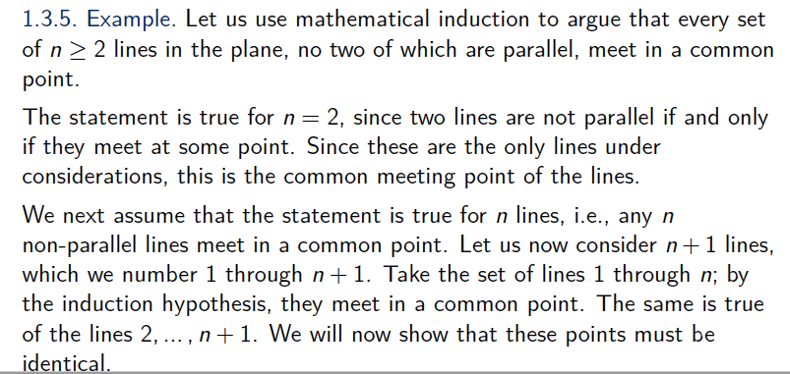
\includegraphics[width=1\textwidth]{induction_1.png}
    \end{figure}
\end{frame}
\begin{frame}
    \frametitle{Induction¿}
    \hspace{1em}
    A strange example shared by Horst. What's going wrong?
    \begin{figure}
        \centering
        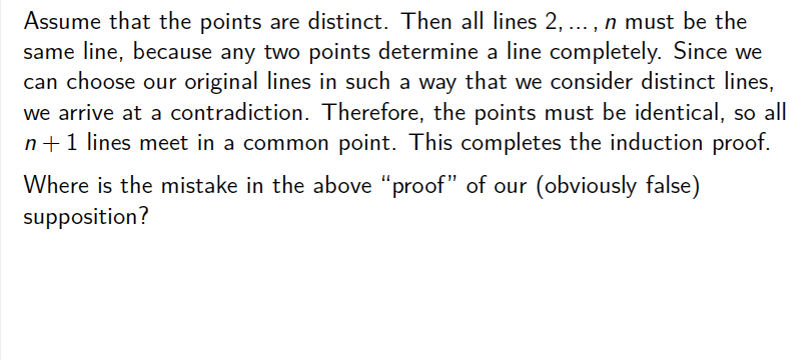
\includegraphics[width=1\textwidth]{induction_2.png}
    \end{figure}
\end{frame}
\begin{frame}
    \frametitle{Exercise}
    3. Let $ a_n$ be the following expression with $n$ nested radicals:\
    $$a_n=\sqrt{2+\sqrt{2+\cdots+\sqrt{2+\sqrt{2}}}}$$
    Please find the explict formula for $a_n$.
\end{frame}
\begin{frame}
    \frametitle{Solution}
    \hh Note that $a_n$ can be defined recursively like this: $a_1 =\sqrt{2}$, and
    $a_{n+1} =\sqrt{a_n+2}$ for $n \geq 1$. We proceed by induction. \\
    \red{Hypothesis:} $a_n= 2 \cos \frac{\pi}{2^{n+1}}$\\
    \red{Base case:} $a_1=\sqrt{2}$, and $2\cdot \cos \frac{\pi}{4}= 2\cdot \frac{1}{\sqrt{2}}=\sqrt{2}$.\\ 
    \red{Inductive case:} assuming the \textbf{\red{IH}} is true for n, then 
    \begin{equation*}
    \begin{aligned}
        a_{n+1}&=\sqrt{2+a_n}=\sqrt{2+2\cos \frac{\pi}{2^{n+1}}}\\
               &=\sqrt{2+2\cos \frac{2\pi}{2^{n+2}}}\\
               &=\sqrt{2+2(2\cos^2\frac{\pi}{2^{n+2}}-1)}\\
               &=\sqrt{4\cos ^2\frac{\pi}{2^{n+2}}}
               =2\cos \frac{\pi}{2^{n+2}}
    \end{aligned}
    \end{equation*}
    By  induction, we conclude that $a_n = 2 \cos \frac{\pi}{2^{n+1}}$.
\end{frame}
\begin{frame}
    \frametitle{Structual Induction}
    \hh Let $B$ be a set and let $C_1, ..., C_n$ be construction rules. 
    Let $B$ be recursively defined to be the $\subseteq$-least set such that 
    $B \subseteq A$ and $A$ is closed under the rules $C_1, ..., C_n$. 
    Let $P(x)$ be a property. If
    \begin{enumerate}
        \item for all $b \in B$, $P(b)$ holds
        \item for all $a_1, ..., a_m$ and $c$ and $1\leq i\leq n$, 
        if $P(a_1), ..., P(a_m)$ all hold and $c$ is obtained from 
        $a_1, ..., a_m$ by a single application of the rule $C_i$, 
        then $P(c)$ holds
    \end{enumerate}
    Then $P(x)$ holds for every element in A.
\end{frame}
\begin{frame}
    \frametitle{Exercise}
    Taken from Ve203 FA 2020 assignment 2: 
    \\ \vs{2em}
    4. Let $S \subset \bN$ be defined by
    \begin{itemize}
        \item $(0,0)\in S$
        \item $(a,b)\in S \Rarrow \left(\left(\left(a+2,b+3\right)\in S\,\right)\wedge \left(\left(a+3,b+2\right)\in S\,\right)\right)$ 
    \end{itemize}
    Use structural induction to show that $(a, b) \in S$ implies $5 \mid (a + b)$.
    \\\textbf{(3 Marks)}
\end{frame}
\section{DNF \& CNF}
\begin{frame}
    \frametitle{DNF \& CNF}
    \yellow{Definition:}
    \begin{itemize}
        \item  CNF: \textbf{product of sums} or an \textbf{AND of ORs}
        \item  DNF: \textbf{sum of products} or an \textbf{OR of ANDS}
    \end{itemize}
    \textcolor[rgb]{0.95,0.75,0.95}{Examples:}
    \begin{itemize}
        \item $(\neg p \vee  q \vee r) \wedge (\neg q \vee \neg r) \wedge (r)$
        \item $(\neg p \wedge q \wedge r) \vee (\neg q \wedge \neg r) $        
    \end{itemize}
    \begin{block}{Question}
        What's the DNF/CNF for a tautology?
    \end{block}
\end{frame}
\begin{frame}
    \frametitle{Exercise}
    5. Suppose that a truth table in \textbf{n} propositional variables 
    is specified. Show that a compound proposition with 
    this truth table can be written to a well-determined DNF. \\(Take from Vv186 Assignment Exercise 1.4)
    \begin{table}[H]
        \begin{tabular}{ccc}
        $A$& $B$ &$f~(A,B)$  \\
        \toprule
        $T$ &$T$  & $T$ \\
        $T$ &$F$  & $F$ \\
        $F$ &$T$  & $T$ \\
        $F$ &$F$  & $F$ \\
        \bottomrule
        \end{tabular}
    \end{table}
    \vv
    $$f~(A,B)=(A \wedge B) \vee (\neg A \wedge B)$$
\end{frame}
\begin{frame}
    \frametitle{Introduction to boolean algebra}
    \vv
    If we regard $\vee$ as $+$, $\wedge$ as $\cdot$, then the equation 
        $$A\wedge(B\vee C)=(A\wedge B)\vee(A\wedge C)$$
    is just the distributivity law:
        $$A \cdot (B+C) = (A\cdot B) + (A \cdot C)$$
    \vv
    \textbf{\textit{\red{Do It Yourself:}}}\\
    Check whether the axiom P1 -- P9 for rational numbers also hold for such operations.
\end{frame}
\begin{frame}
    \frametitle{Properties}
    \hh
    We denote $\neg A$ as $\conj{A}$.
    And, 1 means true ($\top$), 0 means false ($\bot$). 
    We have the following: \vv
    \begin{itemize}
        \item $A \cdot 1 = A$
        \item $A + 1 = 1$
        \item $A + \conj{A} = 1$
        \item $A \cdot \conj{A} = 0$
        \item $\conj{\conj{A}}=A$
        \item $\conj{A+B}=\conj{A}\cdot \conj{B}$
        \item $\conj{A\cdot B}=\conj{A}+ \conj{B}$
        \item \blue{$A+AB=A$}
        \item $\dots$
    \end{itemize}

\end{frame}
\begin{frame}
    \frametitle{A Truth Table}
    \begin{table}[]
        \begin{tabular}{||c|c|c||c||}
        \toprule
        \multicolumn{1}{||c|}{$A$} & \multicolumn{1}{c|}{$B$} & \multicolumn{1}{c||}{$C$} & \multicolumn{1}{c||}{$F(A,B,C)$} \\ 
        \midrule
        T  &  T &  T &  T  \\
        T  &  T &  F &  T  \\
        T  &  F &  T &  F  \\
        T  &  F &  F &  F  \\
        F  &  T &  T &  T  \\
        F  &  T &  F &  F  \\
        F  &  F &  T &  T  \\
        F  &  F &  F &  F  \\
        \bottomrule
        \end{tabular}
        \end{table}
    Expression in DNF:
        $$F = ABC + AB\conj{C} + \conj{A} BC + \conj{A}\,\conj{B}C$$
    \red{Ugly! How to simplify?}
\end{frame}
\section{*Extra Topic}
\begin{frame}
    \frametitle{Gray Code}
    \hh
    In the encoding of a set of binary numbers, 
    if any two adjacent codes differ by \textbf{only one} binary digit, 
    the encoding is called a \blue{gray code}.\\
    \hh Interestingly, there's also only a \textbf{one-digit difference}
     between the largest and the smalleset number, namely \textbf{end to end}.
     \begin{table}[]
        \begin{tabular}{|c|c|c|c|}
        \toprule
        number & code & number & code \\ 
        \midrule
        0 & 0000 & 8 & 1100 \\ \hline
        1 & 0001 & 9 & 1101 \\ \hline
        2 & 0011 & 10 & 1111 \\ \hline
        3 & 0010 & 11 & 1110 \\ \hline
        4 & 0110 & 12 & 1010 \\ \hline
        5 & 0111 & 13 & 1011 \\ \hline
        6 & 0101 & 14 & 1001 \\ \hline
        7 & 0100 & 15 & 1000 \\ 
        \bottomrule
        \end{tabular}
        \end{table}
\end{frame}
\begin{frame}
    \frametitle{How to transfer?}
    \yellow{Binary code -> Gray code (coding) :} \\
    \hh From the rightmost bit, each bit XOR with the left, as the value of the corresponding gray code, 
    the leftmost bit remains unchanged.
    \\
    \vv 
    \red{Gray code - > binary code (decoding) :} \\
    \hh From the second digit on the left, each bit XOR with the decoded value of the left bit,
     as the decoded value of that bit, the leftmost bit remains unchanged.  
    \vv
     \begin{block}{Example}
        \hh \url{https://vijos.org/p/1176}
    \end{block}
\end{frame}
\begin{frame}
    \frametitle{Karnaugh Graph}
    \begin{table}[H]
        \begin{tabular}{||c|c|c|c|c||}
        \hline
        \multicolumn{1}{||r|}{\diagbox{\*$A$}{$BC$}} & 00 & 01 & 11 & 10 \\ 
        \hline
         00 &  &  &\cellcolor[rgb]{0.8,0,0}{1}  &\cellcolor[rgb]{0.8,0,0}{1}  \\ \hline
         01 & \cellcolor[rgb]{0,0.4,0.7}{1} &  &\cellcolor[rgb]{0.8,0,0}{1}  & \cellcolor[rgb]{0.8,0.4,0.7}{1} \\ 
        \hline
        \end{tabular}
        \caption{Karnaugh Graph of 3 variables}
    \end{table}
    Expressions:
    \begin{equation*}
        \begin{aligned}
            F&= \conj{A}BC+ \conj{A} B\conj{C} + A\conj{B}\,\conj{C} + ABC + AB \conj{C}\\
             &= A \conj{C} + B
        \end{aligned}
    \end{equation*}
\end{frame}
\newcommand{\cc}[1]{\overline{#1}}
\begin{frame}
    \frametitle{Exercise}
    5. Simplify the following expressions:
    \begin{itemize}
        \item[a)] $wxyz+wxy\conj{z}+wx\cc{y}\,\conj{z}+w\cc{x}yz+w\cc{x}\,\cc{y}z+w\cc{x}\,\cc{y}\,\cc{z}+\cc{w}x\cc{y}z+\cc{w}\,\cc{x}yz+\cc{w}\,\cc{x}y\cc{z}$ 
        \item[b)] $wx\cc{y}\,\cc{z}+w\cc{x}yz+w\cc{x}y\cc{z}+w\cc{x}\,\cc{y}\,\cc{z}+\cc{w}x\cc{y}\,\cc{z}+\cc{w}\,\cc{x}y\cc{z}+\cc{w}\,\cc{x}\,\cc{y}\,\cc{z}$
    \end{itemize}
    \begin{table}[H]
        \begin{tabular}{||c|c|c|c|c||}
        \hline
        \multicolumn{1}{||r|}{\diagbox{$wx$}{$yz$}} & 00 & 01 & 11 & 10 \\ 
        \hline
         00 &\cellcolor[rgb]{1,0.5,0.1}{1}  &  &  &\cellcolor[rgb]{1,0.5,0.1}{1}  \\ \hline
         01 & &  &  &  \\ \hline
         11 &  &  &  & \\ \hline
         10 &\cellcolor[rgb]{1,0.5,0.1}{1} & & &\cellcolor[rgb]{1,0.5,0.1}{1} \\
         \hline
        \end{tabular}
        \caption{$x\cc{z}=wxyz+wx\cc{y}z+\cc{w}xyz+\cc{w}x\cc{y}z$}
    \end{table}
    Answer: a) $wxyz+wx\cc{z}+w\cc{x}\,\cc{y}+\cc{w}\,\cc{x}y+ \cc{w}x\cc{y}z$\\
    \hs{3.6em} b) $\cc{y}\,\cc{z}+w\cc{x}y+\cc{x}\,\cc{z}$
\end{frame}
\begin{frame}
    \frametitle{OR \& AND in circuits}
    \begin{figure}
        \centering
        %\pgfuseimage{or_circuit}
        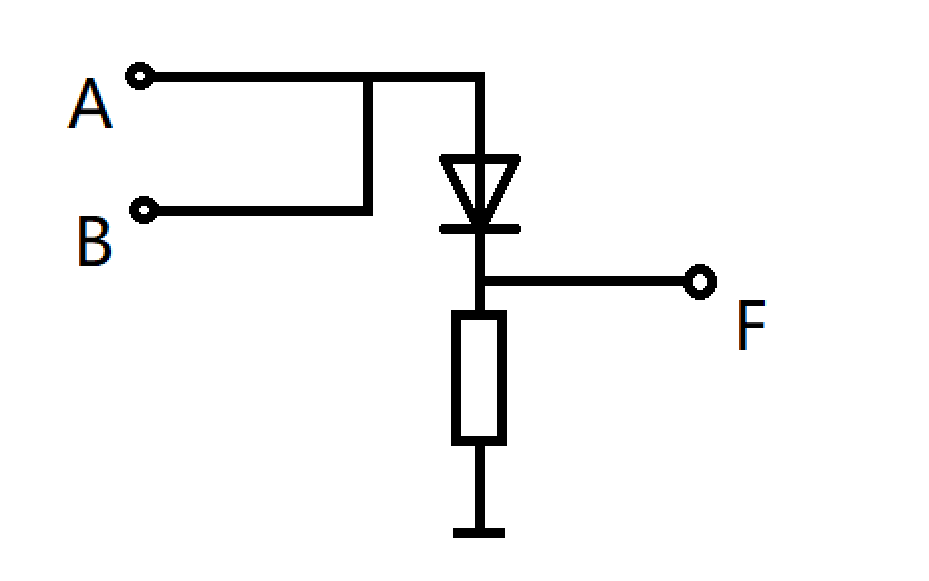
\includegraphics[width=0.6\textwidth]{or_circuit_1.png}
        \caption{OR circuit}
    \end{figure}
    What about AND and NOT ?
\end{frame}
%\begin{frame}
%    \frametitle{Conceptual diagram}
%    \usetikzlibrary{mindmap}
%    \begin{tikzpicture}[mindmap, concept color=blue!60]
%        \node [extra concept] {Statement}
%            child[concept color=red!50,grow=30] {node[concept] (c1) {Statement structure}}
%            child[concept color=orange!50,grow=0] {node[concept] {vacuous truth}};
%        \node [extra concept] at (3,-2) {Sets}
%            child[concept color=green!50, grow=0] {node[concept] {operations}};
%        \node [extra concept] (c2) at (8,1) {Logical operators};
%        \node [extra concept] (c3) at (9,3) {Truth Table};
%        \begin{pgfonlayer}{background}
%            \draw [extra concept connection] 
%                                           
%                                        (c2) edge (c3);
%            \end{pgfonlayer}
%    \end{tikzpicture}
%\end{frame}


\begin{frame}
    \frametitle{Reference}
    \begin{itemize}
        \item Pictures from Dr. Horst Hohberger.
        \item Exercises from 2020-Ve203 Assignment2.
        \item Exercises from 2021-Vv186 Assignment1.
        \item Exercises from 2019--Vv186 TA-Zhang Leyang.
        \item Contents from 2020 Fall Ve203 TA-Peng Chengjun.
        \item Exercises from 2021 Fall Ve203 TA-Zhao Jiayuan.
        \item Exercises from my 2021--Vv186 Mid1 RC.
        \item Kenneth, H.Rosen. Translated by Xu Liutong etc. \itshape Discrete Mathematics amd Its Applications\myfont, 
                 Eightth Edition, Chinese Abridgement. China Machine Press, 2019 print.
    \end{itemize}
\end{frame}
\end{document}